\chapter{Introducción}\label{cap.introduccion}
En este capítulo se introducirá el contexto en el que se sitúa este proyecto y la motivación que ha llevado a su desarrollo. Para ello, es preciso comenzar con una
explicación a grandes rasgos sobre la \acrfull{va}, aprendizaje profundo y la robótica educativa pues es la intersección entre esos campos donde se ubica este \acrfull{tfm}.
\section{Visión artificial y aprendizaje profundo}

Desde la antigüedad el ser humano ha soñado con crear máquinas capaces de pensar. Cuando surgieron los primeros ordenadores programables, las personas se plantearon la idea de lograr que estos computadores adquirieran inteligencia, consiguiendo capacidades empleadas para realizar tareas propias de los humanos. Algunos ejemplos de estas tareas son entender el habla o las imágenes, y automatizar tareas rutinarias. El campo que desarrolla estas tareas se denomina \acrfull{ia}~\cite{Goodfellow} y cada vez tiene más presencia en temas de investigación.\\

En \acrshort{ia} existen diversos desafíos muy interesantes; sin embargo, en la mayoría de ellos es extremadamente difícil alcanzar el rendimiento y la eficiencia del cerebro humano. Las máquinas nos superan en tareas como procesamiento de gran cantidad de datos, almacenamiento de información o tareas de razonamiento como el juego de ajedrez. Sin embargo, algunas habilidades que el ser humano realiza inconscientemente, como caminar o ver, son aún muy complejas para las máquinas.\\

La \acrshort{ia} comprende diferentes campos: \textit{Machine Learning}, incluyendo \textit{Knowledge Engineering}, \acrfull{rna}~\cite{rna}, procesamiento del lenguaje natural, Minería de datos, \acrfull{va}, etc. Este proyecto se enfoca en la \acrshort{va}, que trata de analizar y procesar imágenes de tal forma que un ordenador sea capaz de interpretar dichas imágenes. La \acrshort{va} intenta conseguir que una máquina realice el mismo proceso que el Sistema Visual Humano de tal forma que sea capaz de tomar decisiones y actuar en función de la situación en que se encuentre.\\

El aprendizaje de las máquinas es un punto de encuentro de diferentes disciplinas que engloba a la estadística, la programación y la optimización, entre otras. La \acrshort{va} intenta simular las capacidades del ojo y el cerebro humanos y en ella se utilizan comúnmente técnicas de aprendizaje máquina.\\

Uno de los problemas que se está estudiando ampliamente en \acrshort{va} en la última década es la conducción autónoma. Los humanos somos capaces de mirar a la carretera y saber al instante si el coche que conducimos está en una curva o una recta, si hay coches alrededor y cómo interactúan entre ellos. En función a la situación en la que nos encontramos sabemos qué acciones llevar a cabo para lograr una buena conducción.  Sin embargo, este procedimiento es más complicado para los ordenadores. En la actualidad se está investigando ampliamente cómo emplear las \acrfull{rna} para materializar comportamiento autónomo en vehículos.\\

Un claro ejemplo es la navegación en robótica (Figura \ref{fig.robot}), donde la visión constituye una capacidad sensorial más para la percepción del entorno que rodea al robot. Generalmente se recurre a técnicas de visión estereoscópica con el fin de reconstruir la escena 3D. En algunas ocasiones se añade algún módulo de reconocimiento con el fin de identificar la presencia de determinados objetos, hacia los que debe dirigirse o evitar. Cualquier información que pueda extraerse mediante \acrshort{va} supone una gran ayuda para el movimiento del robot. \\

\begin{figure}[H]
  \begin{center}
    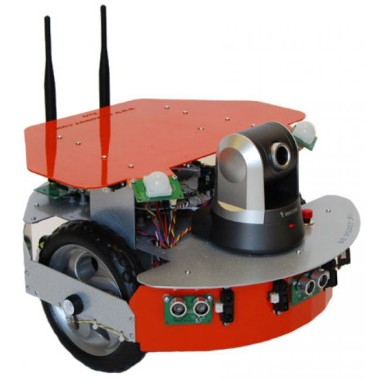
\includegraphics[width=0.3\textwidth]{figures/introduccion/robot.jpg}
		\caption{Navegación en robótica mediante \acrshort{va}}
		\label{fig.robot}
		\end{center}
\end{figure}

La reducción de accidentes gracias a vehículos autónomos es una realidad gracias a la \acrshort{va}, ya que los sistemas de guiado que poseen estos vehículos están basados en esta visión. Algunos ejemplos de estos sistemas (Figura \ref{fig.car}) son: los sistemas de aviso de cambio de carril, o de control de velocidad de crucero. 

\begin{figure}[H]
  \begin{center}
    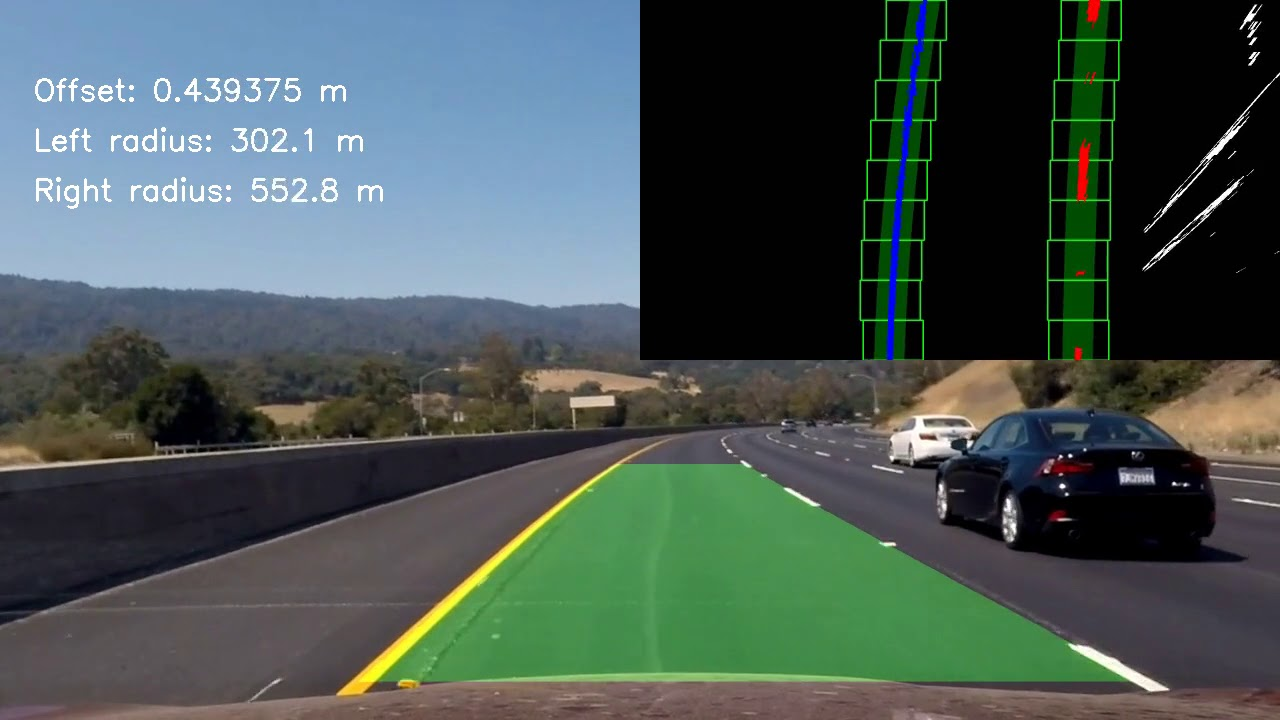
\includegraphics[width=0.5\textwidth]{figures/introduccion/car.jpg}
		\caption{Conducción autónoma}
		\label{fig.car}
		\end{center}
\end{figure}

Otro ejemplo en donde la \acrshort{va} supone un gran avance es la comunidad médica, donde permite diagnosticar con mayor rapidez y detalle enfermedades y lesiones. De esta forma es posible aplicar tratamientos personalizados y eficaces en menor tiempo. Un claro ejemplo de investigadores que emplean \acrshort{va} es el \acrfull{csail}~\cite{cancer}, donde el desarrollo de algoritmos que analizan mamografías de una forma novedosa permite ayudar a detectar el cáncer de mama (Figura \ref{fig.cancer}) con hasta cinco años de anticipación.\\

\begin{figure}[H]
  \begin{center}
    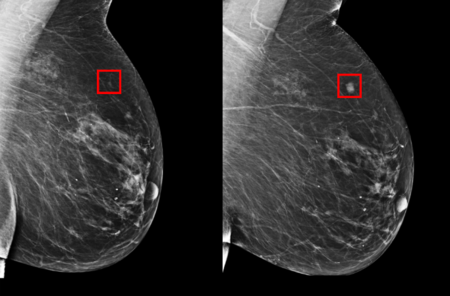
\includegraphics[width=0.4\textwidth]{figures/introduccion/cancer.png}
		\caption{Detección de cáncer de mama}
		\label{fig.cancer}
		\end{center}
\end{figure}


Otra aplicación es el mantenimiento e inventariado urbano. Es posible identificar problemas en instalaciones y mobiliario urbano (averías, mal estado de contenedores (Figura \ref{fig.contenedor}), socavones en la vía pública, etc) mediante cámaras ubicadas por ejemplo en autobuses. Los mantenimientos de infraestructuras de transporte, como vías y cables ferroviarios, pueden programarse automáticamente implantando sistemas de \acrshort{va} en los propios trenes. 


\begin{figure}[H]
  \begin{center}
    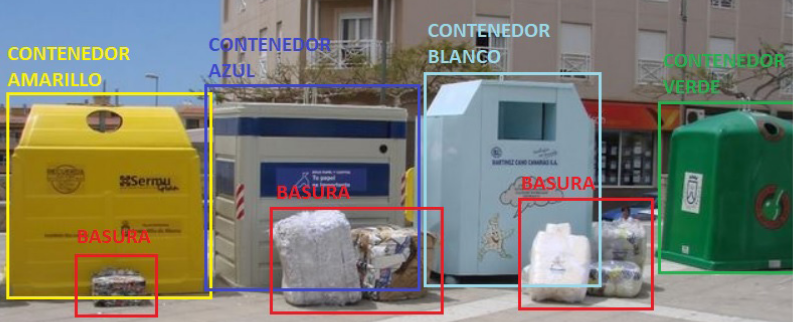
\includegraphics[width=0.5\textwidth]{figures/introduccion/contenedor.png}
		\caption{Detección de contenedores}
		\label{fig.contenedor}
		\end{center}
\end{figure}


\section{Robótica educativa}
La robótica educativa es un campo en auge debido al gran desarrollo de la robótica y la necesidad creciente de especialistas y profesionales en todo el mundo. En 2015, la Comunidad de Madrid introdujo la asignatura “Tecnología, Programación y Robótica” en el plan docente de Enseñanza Secundaria[1]. En el año 2020- 2021 se prevé implantar la asignatura “Programación y Robótica” en el plan docente de Enseñanza Primaria[2]. 

Alineado con la robótica, en los últimos años, está creciendo el interés en la educación \acrfull{stem}. Esta nueva forma de enseñanza promueve el pensamiento científico y la adquisición de conocimientos tecnológicos aplicables a situaciones reales permitiendo el desarrollo de competencias en la resolución de problemas.

Para impartir este tipo de asignaturas es necesaria la infraestructura adecuada. Las plataformas como la de \textit{LEGO} o la de \textit{Arduino} permiten una enseñanza y aprendizaje sencillos de la robótica resultando muy gratificante para el alumno por lo vistoso de los resultados y la obtención de una aplicación real inmediata.\\

Es importante acercar este conocimiento tan complejo de manera adecuada a edades cada vez más tempranas para facilitar un mayor desarrollo en el conocimiento de esta tecnología. Es por ello que cada vez hay más plataformas y entornos \acrshort{stem} que desarrollan software orientado a niños. Algunos ejemplos de plataformas educativas son: 
\begin{itemize}
  \item Scratch\cite{Scratch}. Es un proyecto utilizado en docencia y liderado por el \textit{MIT}\footnote{\url{https://www.mit.edu}} para programar animaciones, interacciones y juegos de manera sencilla por su interfaz visual. Toda la funcionalidad de un lenguaje de programación está embebida en bloques gráficos que agrupan funcionalidades específicas.
  \item LEGO\cite{Lego}. Se trata de una plataforma que dispone de multitud de robots programables también con su sistema gráfico basado en \textit{LabView}\footnote{\textit{LabVIEW} es una plataforma y entorno de desarrollo para diseñar sistemas, con un lenguaje de programación visual gráfico}.
  \item Kodu\cite{Kodu}. Es un sistema de programación visual para el desarrollo de videojuegos desarrollado por Microsoft\footnote{\url{https://www.microsoft.com/es-es}}
  \item Snap!\cite{Snap}. Se trata de un lenguaje visual y una plataforma inspirada en Scratch pero con funcionalidad destinada a edades más avanzadas que permiten el desarrollo de funcionalidad más compleja.
  \item OpenRoberta\footnote{\url{https://lab.open-roberta.org/}} [7]. Es una plataforma educativa en la nube desarrollada por el instituto alemán Fraunhofer IAIS para que los niños puedan programar robots utilizando Lego Mindstorms o robots programables(Figura \ref{fig.roberta})
  \begin{figure}[H]
  \begin{center}
    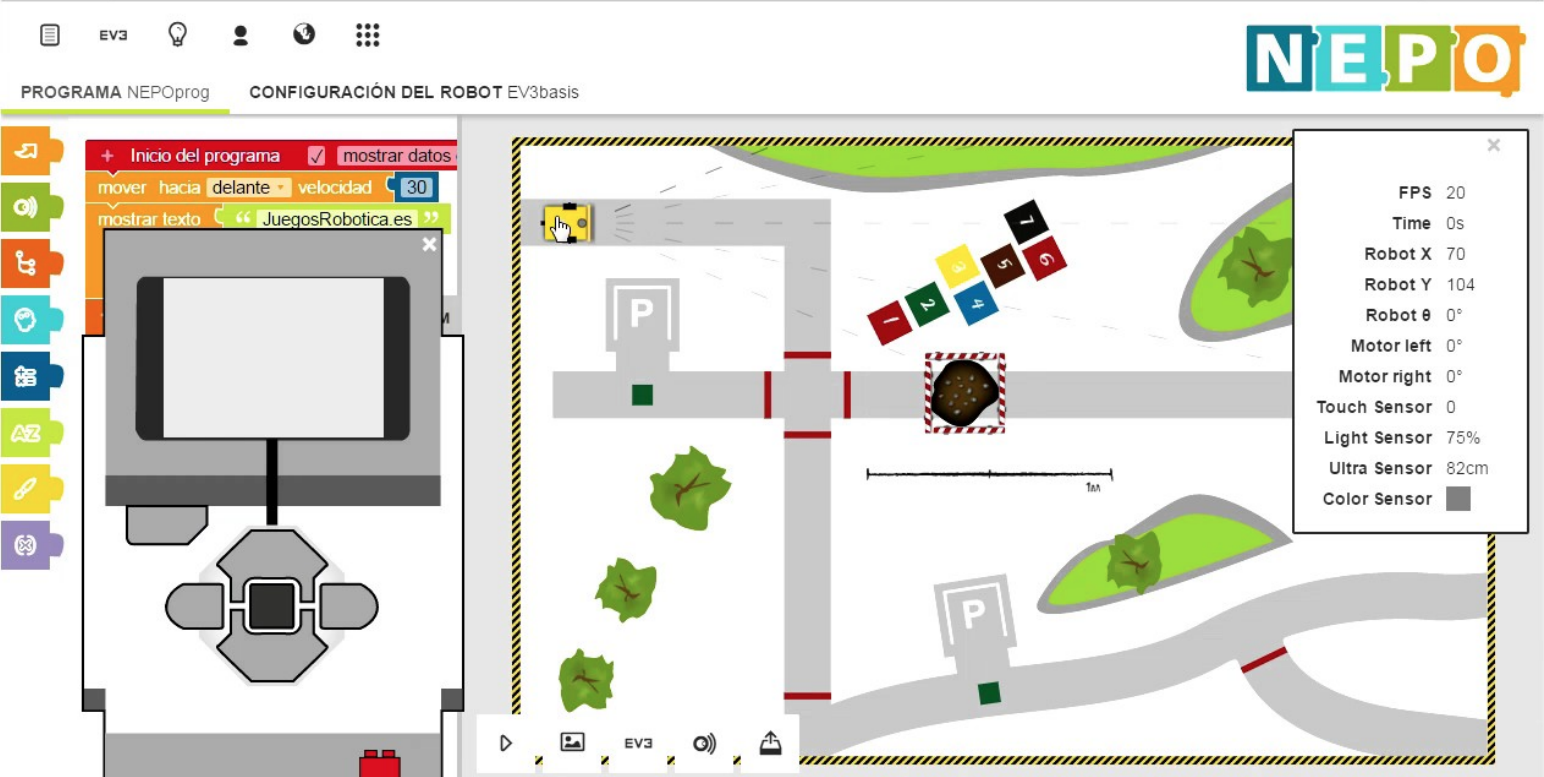
\includegraphics[width=0.5\textwidth]{figures/introduccion/openRoberta.png}
		\caption{Plataforma Open Roberta}
		\label{fig.roberta}
		\end{center}
\end{figure}
  \item Vex\footnote{\url{https://www.vexrobotics.com/}}. Plataforma orientada a la disciplina STEM de enseñanza que ofrece una gran cantidad de robots programables, así como tutoriales para aprender a montarlos y manejarlos. 
  \item AppInventor\footnote{\url{https://appinventor.mit.edu/}}. Es un entorno de desarrollo software creado por Google Labs y actualmente mantenido por el \textit{MIT} que ofrece toda la infraestructura necesaria para crear aplicaciones en Android. De esta manera, y visualmente, el usuario puede desarrollar una aplicación con bloques de código visuales, parecidos a Scratch.
  \item Arduino Web Editor\footnote{\url{https://create.arduino.cc/}}. Arduino Web Editor es una plataforma que proporciona al usuario todo lo necesario para poder programar su código en línea. De esta manera, no es necesario que el usuario instale ningún tipo de software en su sistema. Esto facilita mucho el aprendizaje dado que es inmediato (Figura \ref{fig.arduino})
  
\end{itemize}
 \begin{figure}[H]
  \begin{center}
    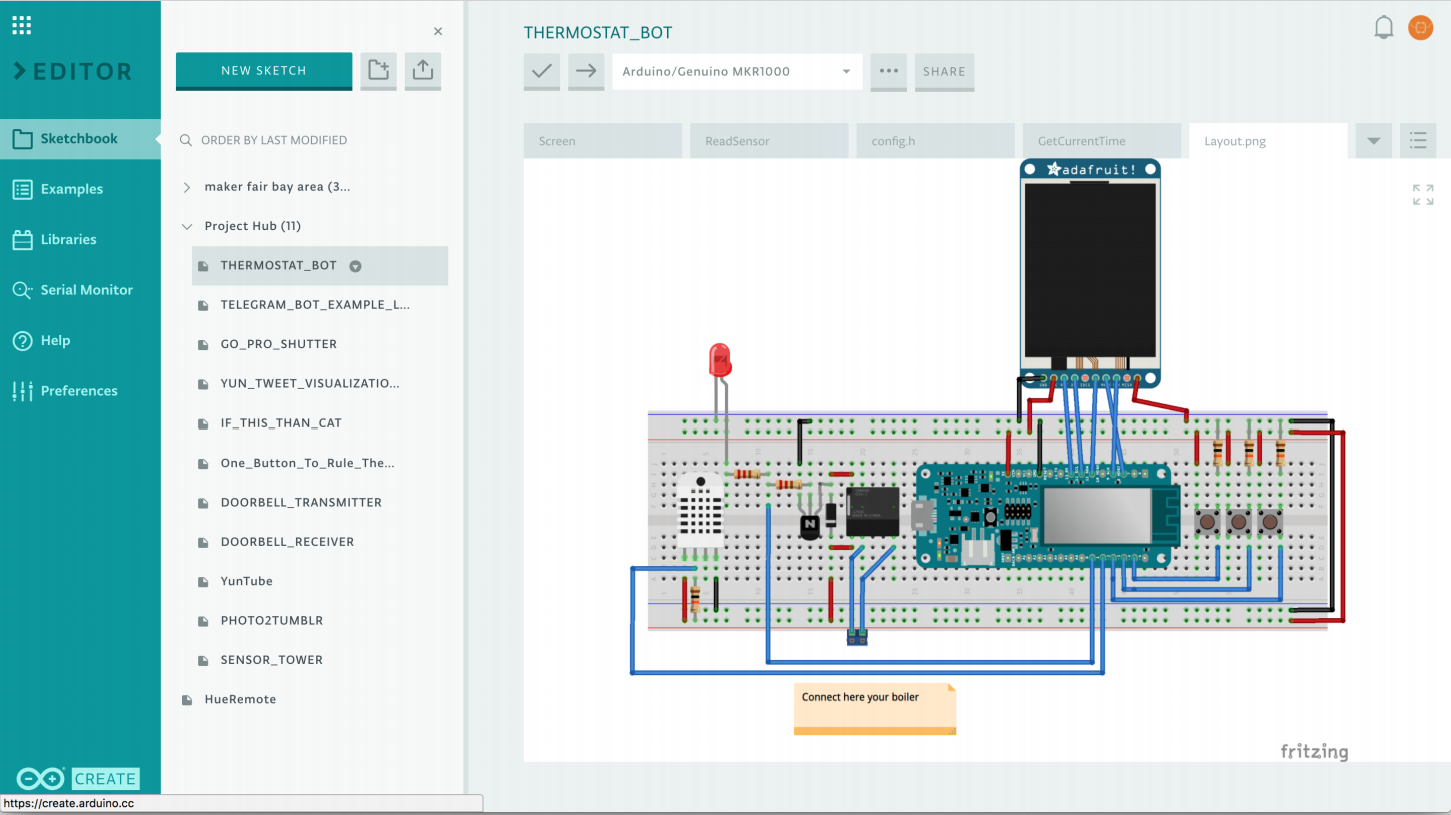
\includegraphics[width=0.5\textwidth]{figures/introduccion/arduino.png}
		\caption{\textit{Arduino} Web Editor}
		\label{fig.arduino}
		\end{center}
\end{figure}
Otra plataforma de robótica educativa, en la que se ha desarrollado este trabajo, es \textit{Kibotics} (Figuras \ref{fig:inKib1} y \ref{fig:inKib2}), que ofrece distintos entornos simulados y con robots reales a los alumnos. Con esto, los alumnos pueden programar la inteligencia de robots autónomos para que realicen distintas pruebas sin ningún riesgo. De esta manera es posible aprender robótica en casi cualquier edad de manera sencilla y con la única necesidad de acceso a internet.
\begin{figure}[!htb]
\minipage{0.45\textwidth}
    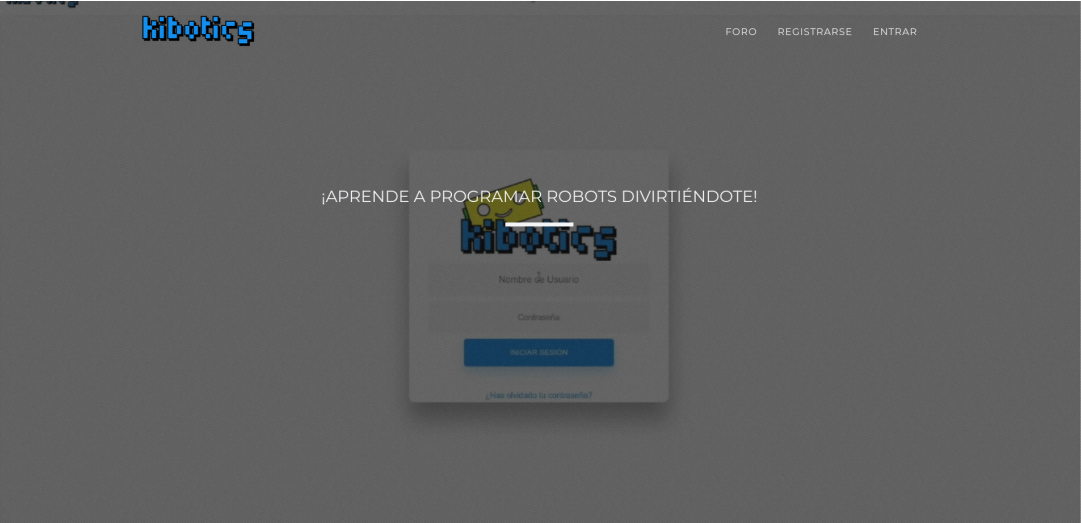
\includegraphics[width=\linewidth]{figures/introduccion/kibotics1.png}
    \caption{Plataforma \textit{Kibotics}}\label{fig:inKib1}
\endminipage\hfill
\minipage{0.45\textwidth}
    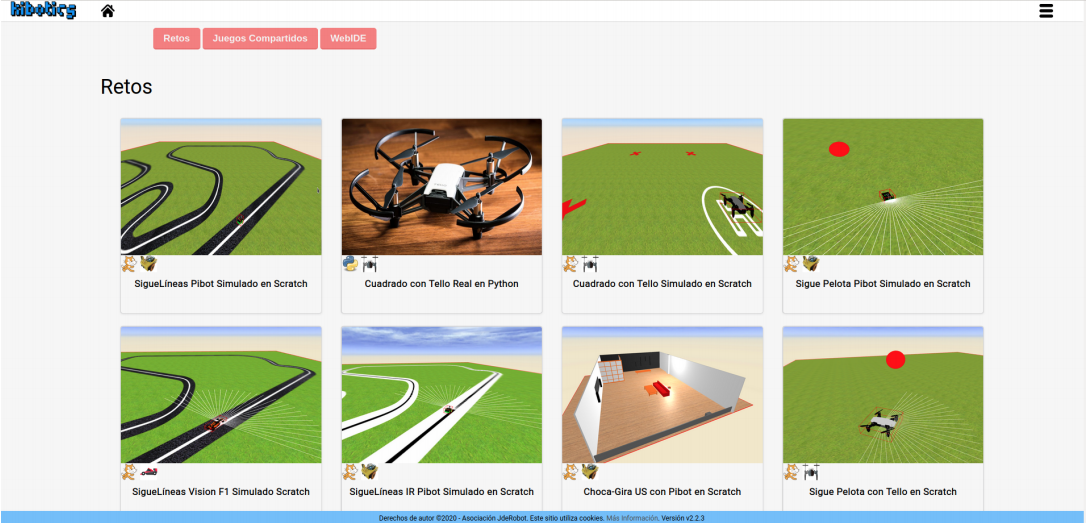
\includegraphics[width=\linewidth]{figures/introduccion/kibotics2.png}
    \caption{Parrilla de ejercicios en \textit{Kibotics}}\label{fig:inKib2}
\endminipage\hfill
\end{figure}


Esta plataforma permite el aprendizaje de la robótica con un simulador en un entorno web. De esta manera, los usuarios sólo necesitan conexión a internet. Soporta distintos modelos de robots como el dron Tello o el Mbot, entre otros, tanto de manera simulada como en los robots reales. Además ofrece dos lenguajes de programación, Scratch (Figura \ref{fig:inKib3}) y Python (Figura \ref{fig:inKib4}) para llegar a usuarios de distintas edades.

 \begin{figure}[!htb]
  \begin{center}
   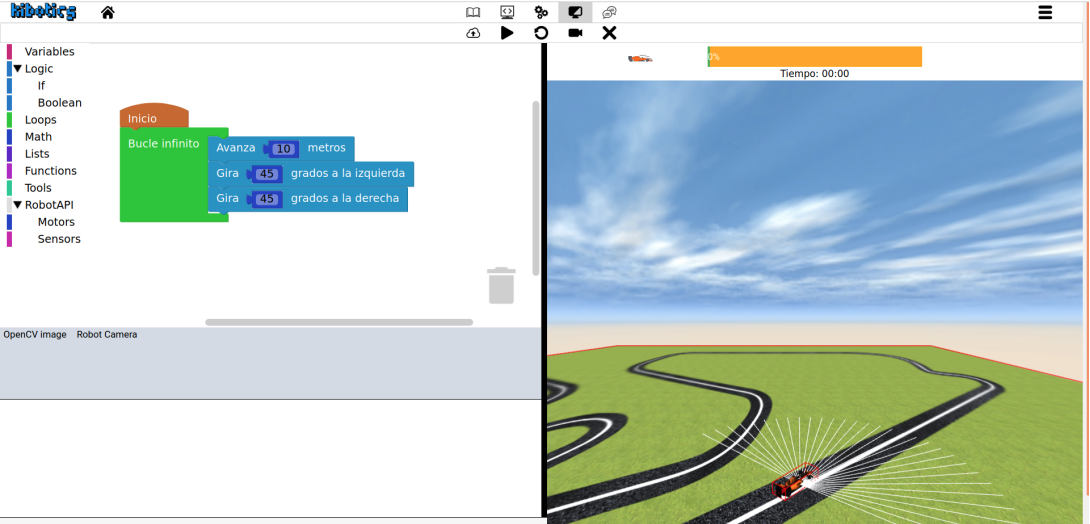
\includegraphics[width=0.9\textwidth]{figures/introduccion/kibotics3.png}
		\caption{Editor y simulador de un ejercicio \textit{Scratch}}
		\label{fig:inKib3}
		\end{center}
\end{figure}

 \begin{figure}[!htb]
  \begin{center}
   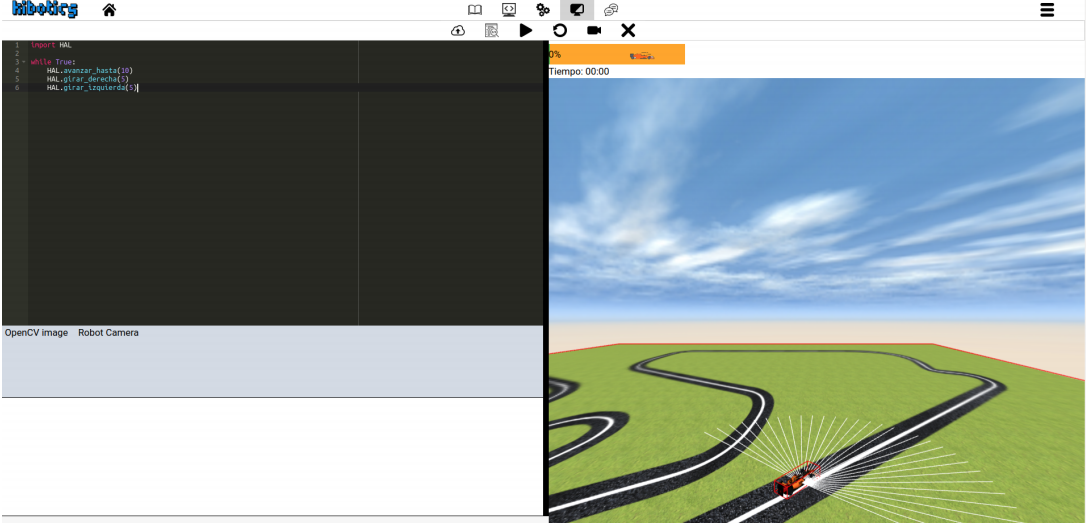
\includegraphics[width=0.9\textwidth]{figures/introduccion/kibotics4.png}
		\caption{Editor y simulador de un ejercicio \textit{Python}}
		\label{fig:inKib4}
		\end{center}
\end{figure}

